\documentclass{beamer}

\usepackage[utf8]{inputenc}
\usepackage{hyperref}

\usetheme{Berkeley}
\beamertemplatenavigationsymbolsempty
\setbeamertemplate{headline}{}
 
\title{Clustering in FoodChain-Lab}
\date{}
 
\begin{document}
\maketitle

\section{Task}
\begin{frame}
	\begin{itemize}
		\item Nutzen sie folgenden Workflow: \url{https://github.com/SiLeBAT/BfROpenLabResources/raw/master/GitHubPages/workflows/Example_Workflow.zip}
		\item Clustern sie alle französischen Station basierend auf dem Attribut "City".
		\item Das bedeutet alle Stationen aus derselben Stadt werden in eine Meta-Station gepackt.
	\end{itemize}
\end{frame}
 
\section{1}
\begin{frame}
	\begin{center}
  		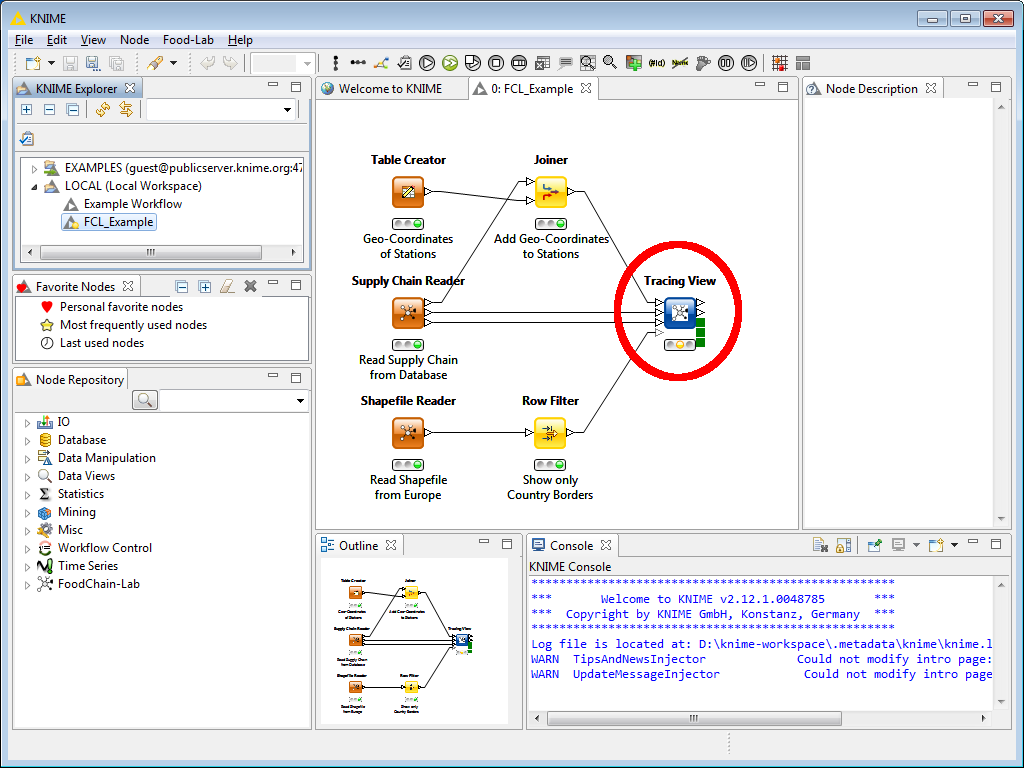
\includegraphics[height=0.6\textheight]{1.png}
	\end{center}
	\begin{itemize}
		\item Importieren sie den Beispiel-Workflow von \url{https://github.com/SiLeBAT/BfROpenLabResources/raw/master/GitHubPages/workflows/Example_Workflow.zip}.
		\item Öffnen sie den \textbf{Tracing View} per Doppelklick.
	\end{itemize}
\end{frame}

\section{2}
\begin{frame}
	\begin{center}
  		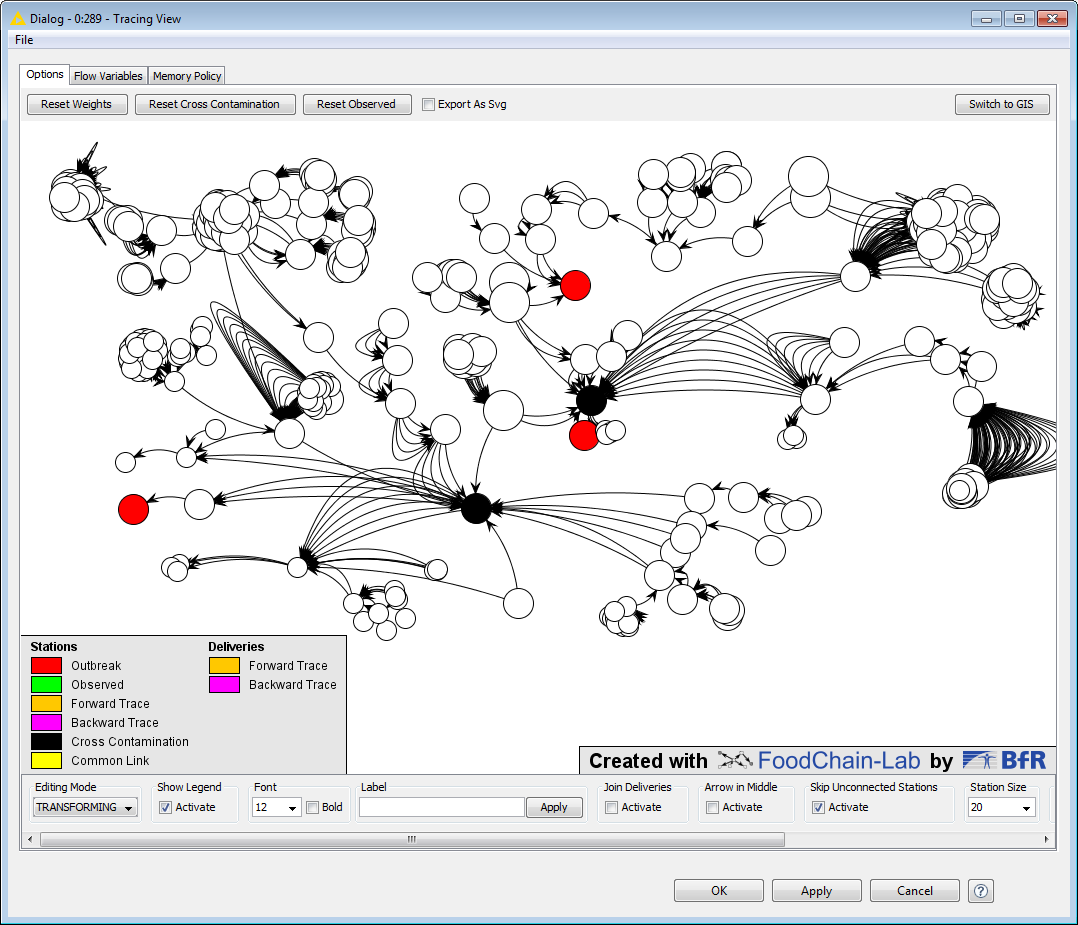
\includegraphics[height=0.6\textheight]{2.png}
	\end{center}
	\begin{itemize}
		\item Ein Fenster mit dem Graphen des Liefernetzes sollte erscheinen.
	\end{itemize}
\end{frame}

\section{3}
\begin{frame}
	\begin{center}
  		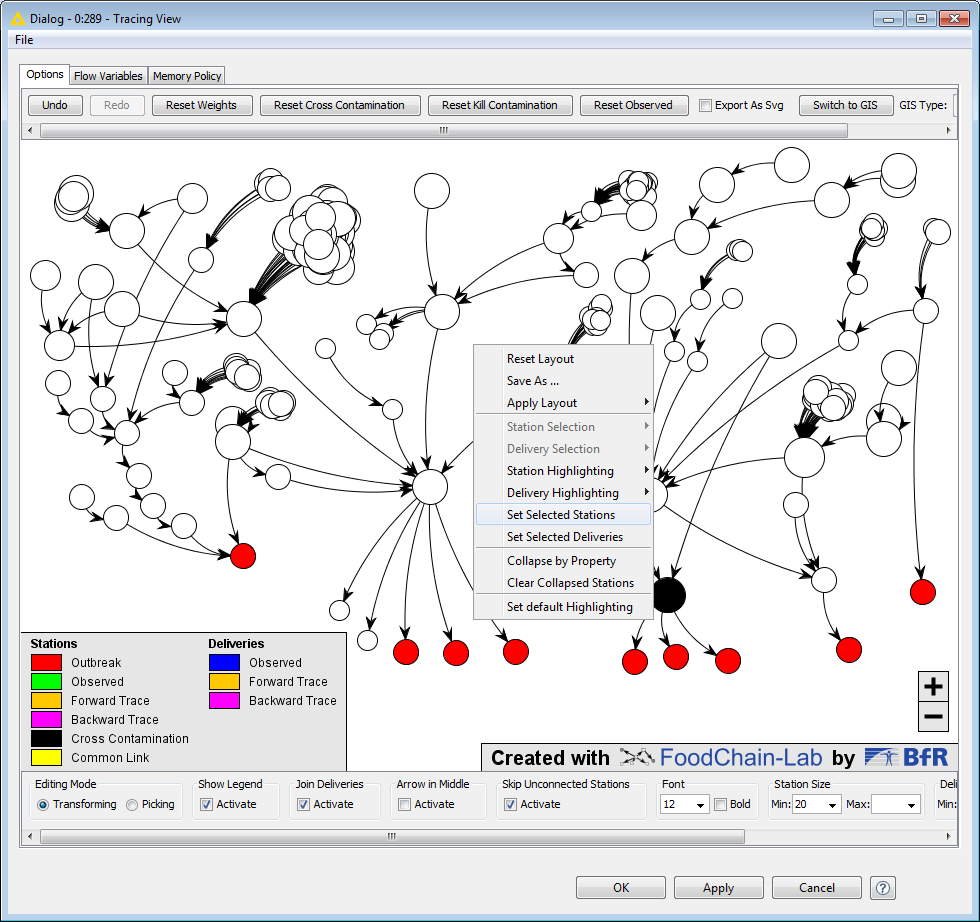
\includegraphics[height=0.6\textheight]{3.png}
	\end{center}
	\begin{itemize}
		\item Machen sie einen Rechtsklick in den Graphen und wählen sie \textbf{Select Stations}.
	\end{itemize}
\end{frame}

\section{4}
\begin{frame}
	\begin{center}
  		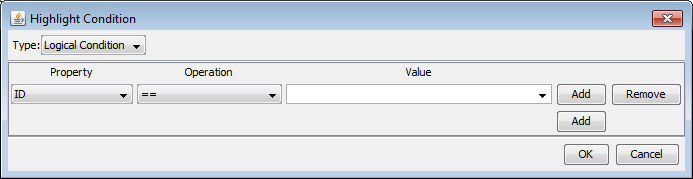
\includegraphics[width=0.9\textwidth]{4.png}
	\end{center}
	\begin{itemize}
		\item Sie sollten jetzt diesen Dialog sehen.
	\end{itemize}
\end{frame}

\section{5}
\begin{frame}
	\begin{center}
  		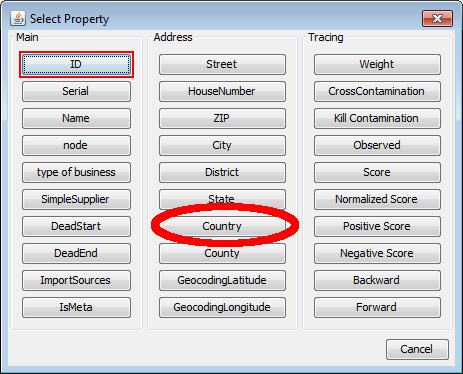
\includegraphics[width=0.9\textwidth]{5.png}
	\end{center}
	\begin{itemize}
		\item Wir möchten alle französischen Station clustern, da die meisten Primärproduzenten in diesem Datensatz aus Frankreich kommen.
		\item Wählen "Country" als \textbf{Property} und "FR" als \textbf{Value} und klicken sie \textbf{OK}.
	\end{itemize}
\end{frame}

\section{6}
\begin{frame}
	\begin{center}
  		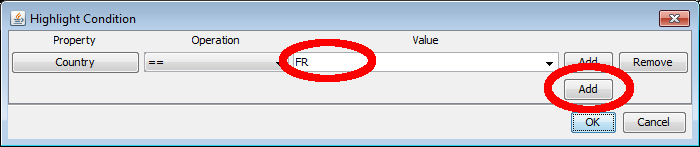
\includegraphics[height=0.6\textheight]{6.png}
	\end{center}
	\begin{itemize}
		\item Alle französischen Stationen sind jetzt selektiert (blau markiert).
	\end{itemize}
\end{frame}

\section{7}
\begin{frame}
	\begin{center}
  		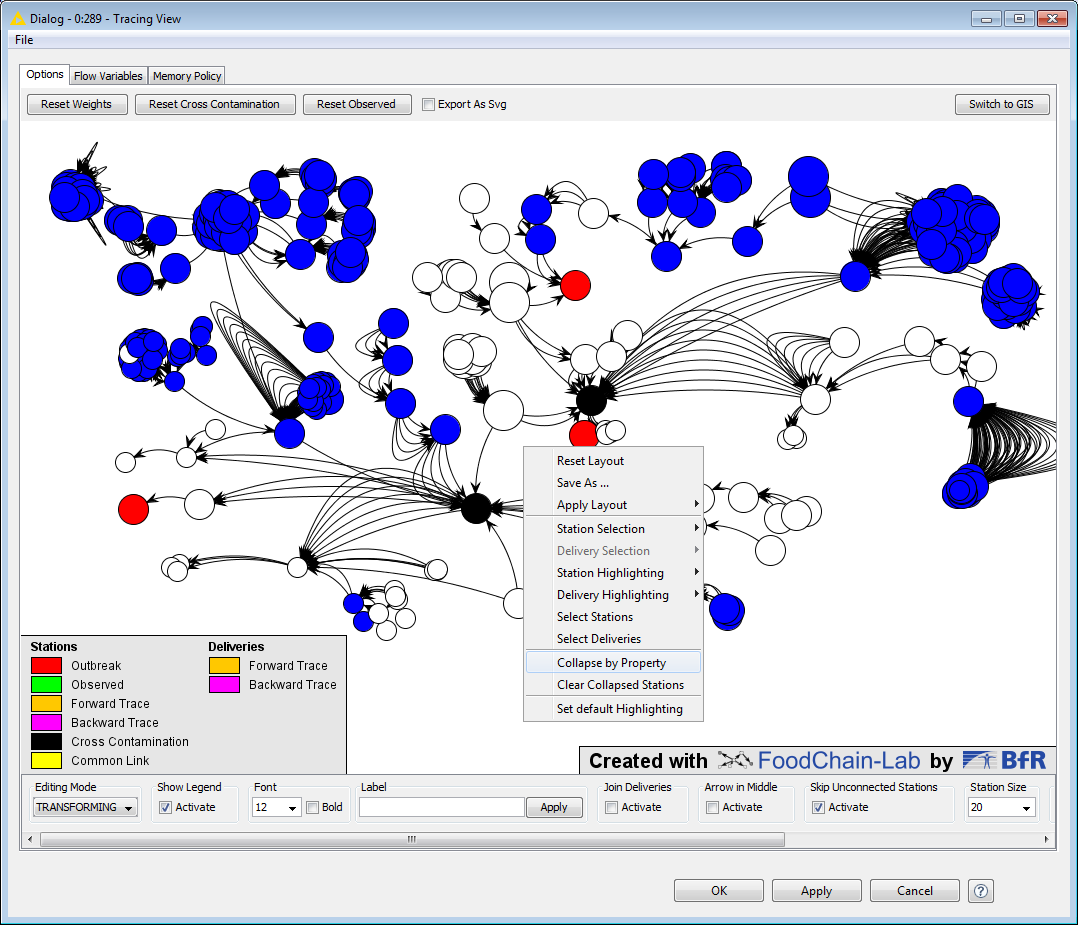
\includegraphics[height=0.6\textheight]{7.png}
	\end{center}
	\begin{itemize}
		\item Machen sie einen Rechtsklick in den Graphen und wählen sie \textbf{Collapse by Property} um die selektierten Stationen zu clustern.
	\end{itemize}
\end{frame}

\section{8}
\begin{frame}
	\begin{center}
  		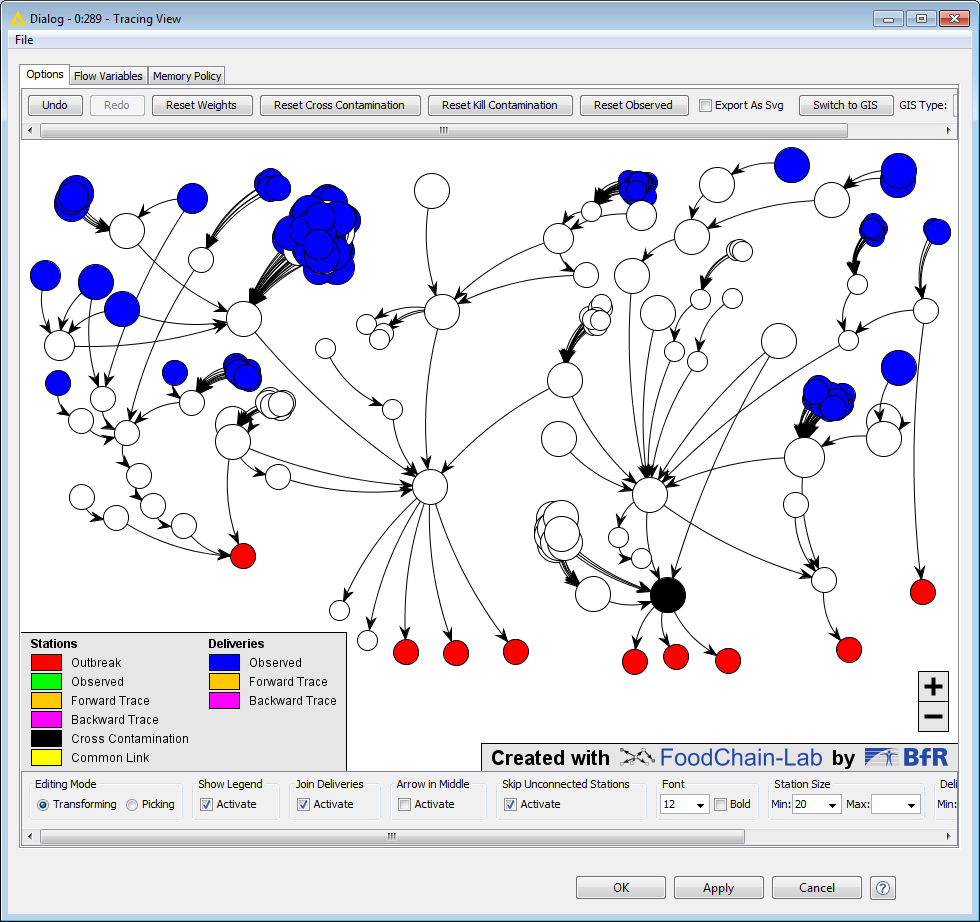
\includegraphics[width=0.7\textwidth]{8.png}
	\end{center}
	\begin{itemize}
		\item Wählen sie \textbf{Yes} um nur die selektierten Stationen fürs Clustern zu nutzen.
	\end{itemize}
\end{frame}

\section{9}
\begin{frame}
	\begin{center}
  		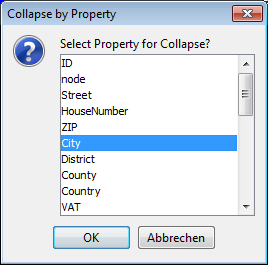
\includegraphics[height=0.5\textheight]{9.png}
	\end{center}
	\begin{itemize}
		\item Da wir auf Basis des Attributs "City" clustern wollen, wählen sie dieses und klicken sie \textbf{OK}.
	\end{itemize}
\end{frame}

\section{10}
\begin{frame}
	\begin{center}
  		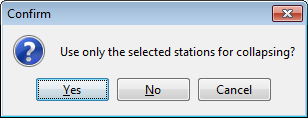
\includegraphics[height=0.5\textheight]{10.png}
	\end{center}
	\begin{itemize}
		\item Klicken sie einfach nur \textbf{OK}, da wir keine Städte ausschließen wollen.
	\end{itemize}
\end{frame}

\section{11}
\begin{frame}
	\begin{center}
  		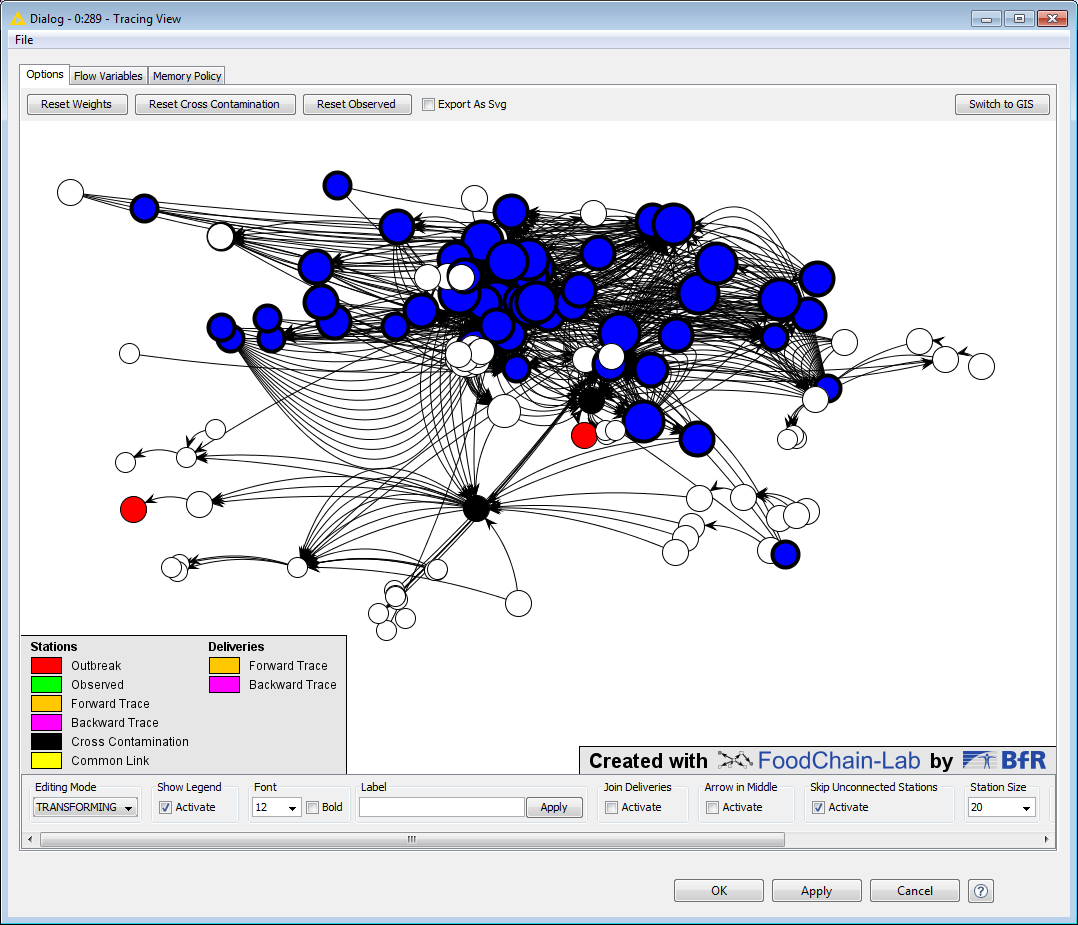
\includegraphics[height=0.6\textheight]{11.png}
	\end{center}
	\begin{itemize}
		\item Alle französischen Station sind nun nach "City" geclustert.
		\item Jede selektierte Meta-Station (blue circle) ist eine französische Stadt.
	\end{itemize}
\end{frame}

\section{12}
\begin{frame}
	\begin{center}
  		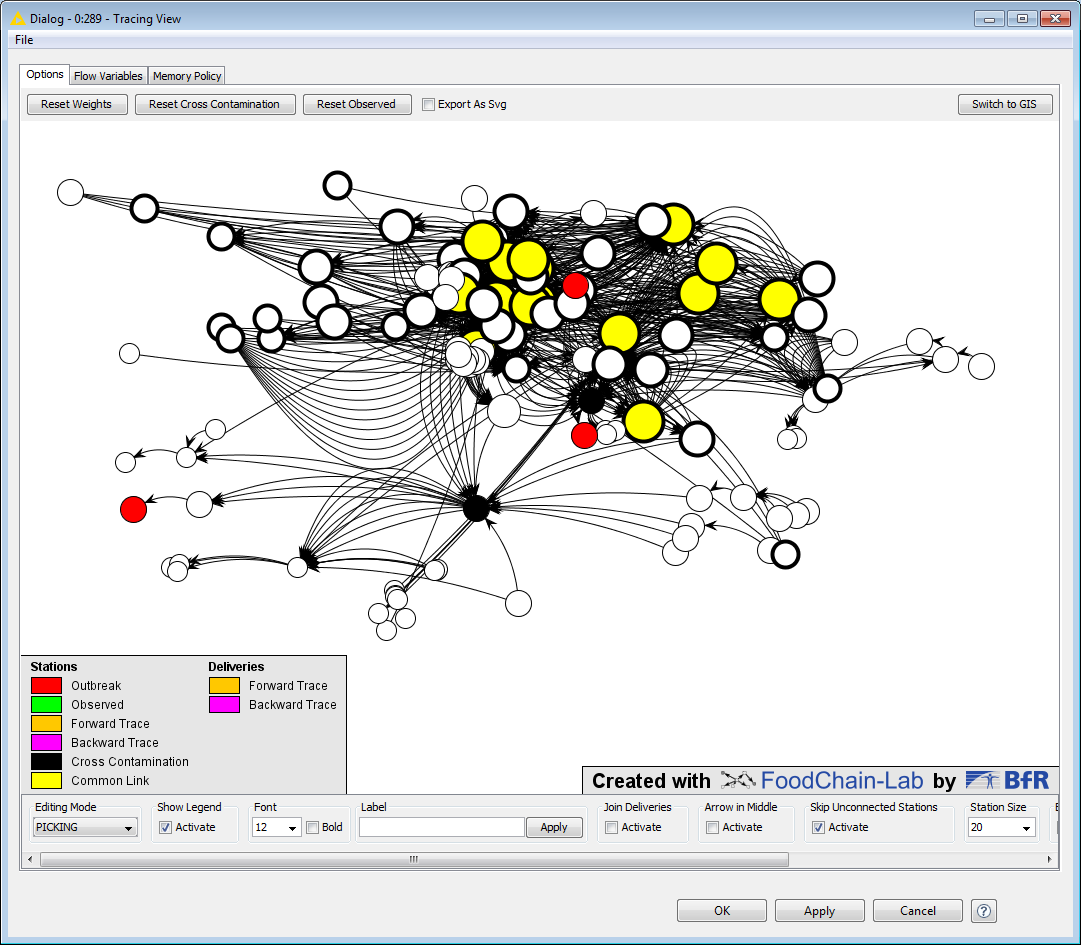
\includegraphics[height=0.6\textheight]{12.png}
	\end{center}
	\begin{itemize}
		\item Wählen sie "PICKING" als \textbf{Editing Mode} and klicken sie an eine leere Stelle des Graphen um alle Station zu deselektieren.
		\item Nun können sie sehen, dass einige der Meta-Station gelb sind. Das bedeutet, dass diese französischen Städte eine Verbindung zu allen Ausbruchs-Stationen haben.
	\end{itemize}
\end{frame}

\section{13}
\begin{frame}
	\begin{center}
  		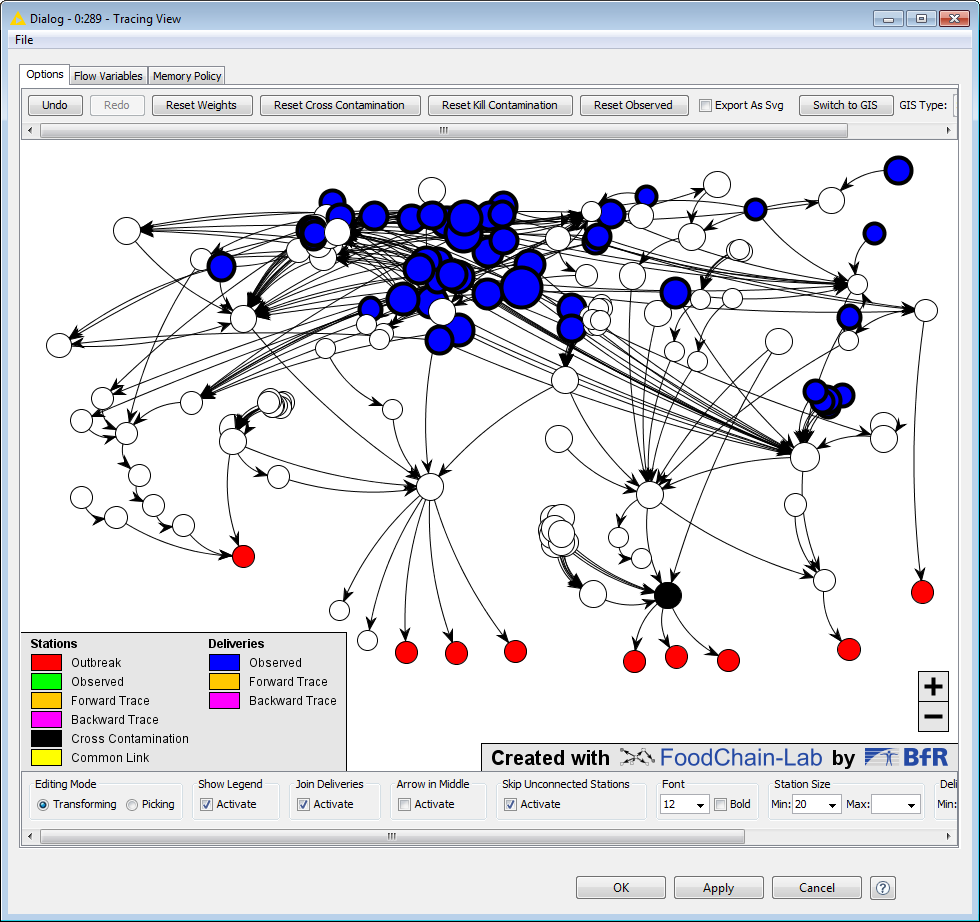
\includegraphics[height=0.6\textheight]{13.png}
	\end{center}
	\begin{itemize}
		\item Da der Graph jetzt recht unübersichtlich aussieht, sollten einen Layout-Algorithmus anwenden.
		\item Machen sie einen Rechtsklick in den Graphen und wählen sie \textbf{Apply Layout $>$ Fruchterman–Reingold}.
	\end{itemize}
\end{frame}

\section{14}
\begin{frame}
	\begin{center}
  		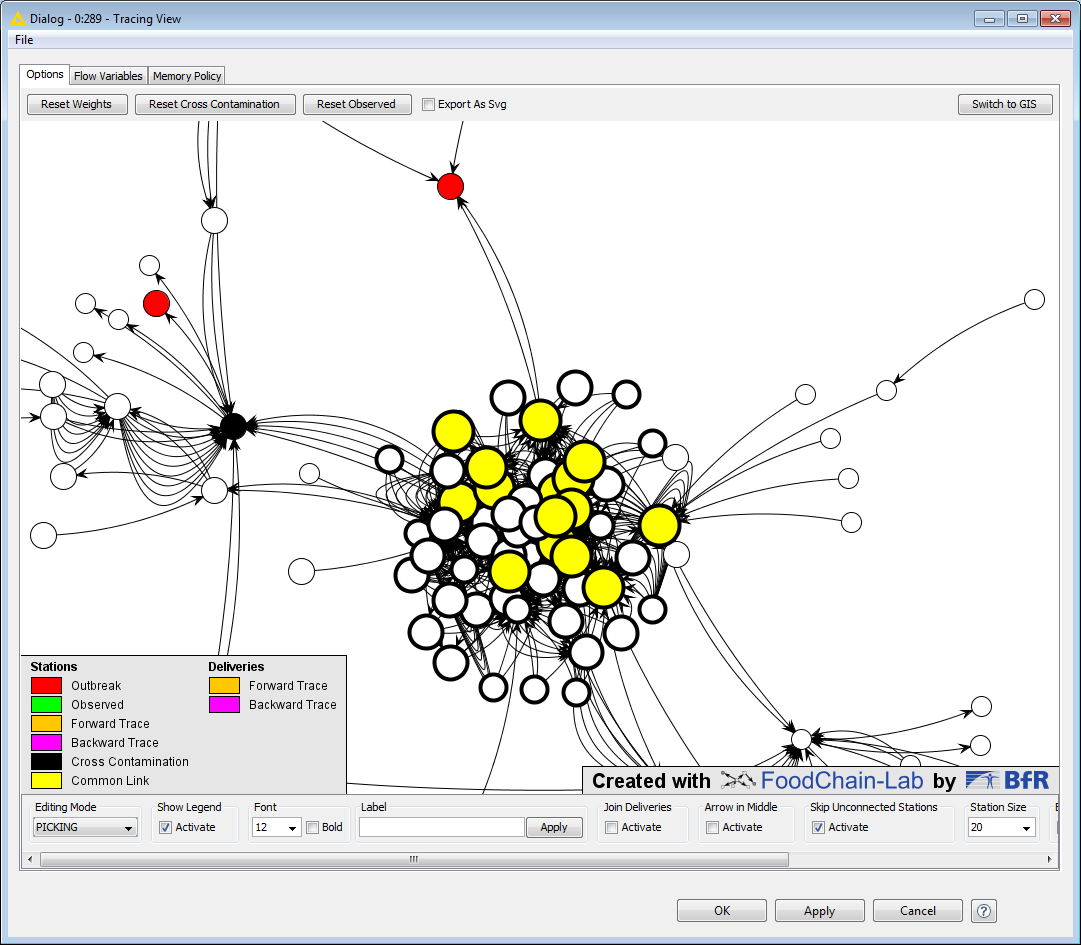
\includegraphics[height=0.6\textheight]{14.png}
	\end{center}
	\begin{itemize}
		\item Der Graph sollte jetzt übersichtlicher angeordnet sein.
		\item Der Algorithmus ist nicht deterministisch. Deshalb wird ihr Graph anders aussehen als der Screenshot hier.
	\end{itemize}
\end{frame}

\section{15}
\begin{frame}
	\begin{center}
  		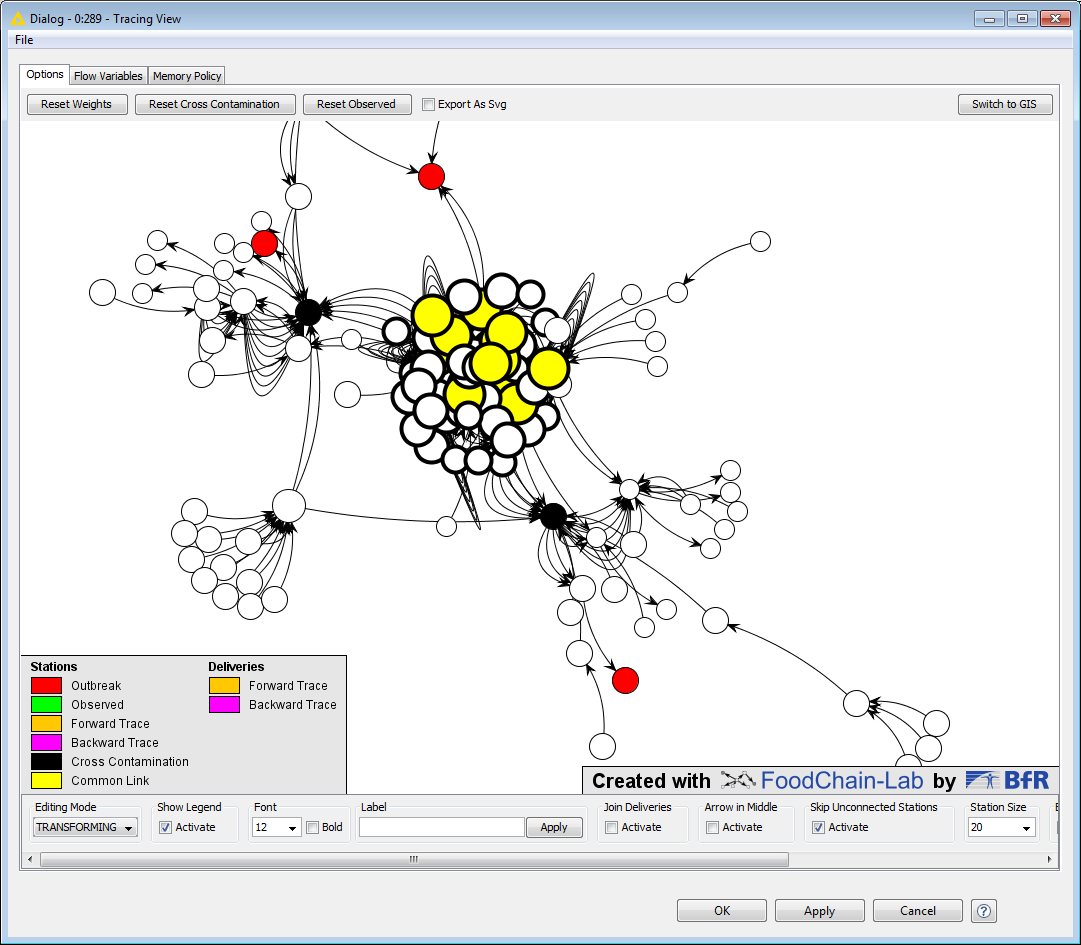
\includegraphics[height=0.6\textheight]{15.png}
	\end{center}
	\begin{itemize}
		\item Nach Anwenden des Layout-Algorithmus sind einige Stationen nicht mehr im sichtbaren Bereich.
		\item Um den ganzen Graphen zu sehen, wählen sie "TRANSFORMING" als \textbf{Editing Mode} and zoomen sie bis sie den ganzen Graph sehen können (Zoomen funktioniert wie in Google Maps).
	\end{itemize}
\end{frame}

\end{document}